\documentclass[conference]{IEEEtran}
\IEEEoverridecommandlockouts
% The preceding line is only needed to identify funding in the first footnote. If that is unneeded, please comment it out.
\usepackage{cite}
\usepackage{amsmath,amssymb,amsfonts}
\usepackage{algorithmic}
\usepackage{graphicx}
\usepackage{textcomp}
\usepackage{xcolor}
\usepackage{hyperref}
\def\BibTeX{{\rm B\kern-.05em{\sc i\kern-.025em b}\kern-.08em
    T\kern-.1667em\lower.7ex\hbox{E}\kern-.125emX}}
\begin{document}

\title{Bithumb Analysis (Temporary title)\\
{\footnotesize \textsuperscript{*}Note: Sub-titles are not captured in Xplore and
should not be used}
\thanks{Identify applicable funding agency here. If none, delete this.}
}

\author{\IEEEauthorblockN{1\textsuperscript{st} Given Name Surname}
\IEEEauthorblockA{\textit{dept. name of organization (of Aff.)} \\
\textit{name of organization (of Aff.)}\\
City, Country \\
email address or ORCID}
\and
\IEEEauthorblockN{2\textsuperscript{nd} Given Name Surname}
\IEEEauthorblockA{\textit{dept. name of organization (of Aff.)} \\
\textit{name of organization (of Aff.)}\\
City, Country \\
email address or ORCID}
\and
\IEEEauthorblockN{3\textsuperscript{rd} Given Name Surname}
\IEEEauthorblockA{\textit{dept. name of organization (of Aff.)} \\
\textit{name of organization (of Aff.)}\\
City, Country \\
email address or ORCID}
}

\maketitle

\begin{abstract}
This document is a model and instructions for \LaTeX.
This and the IEEEtran.cls file define the components of your paper [title, text, heads, etc.]. *CRITICAL: Do Not Use Symbols, Special Characters, Footnotes, 
or Math in Paper Title or Abstract.
\end{abstract}

\begin{IEEEkeywords}
component, formatting, style, styling, insert
\end{IEEEkeywords}

\section{Introduction}
This document is a model and instructions for \LaTeX.
Please observe the conference page limits. 

\section{Ease of Use}

\subsection{Maintaining the Integrity of the Specifications}

The IEEEtran class file is used to format your paper and style the text. All margins, 
column widths, line spaces, and text fonts are prescribed; please do not 
alter them. You may note peculiarities. For example, the head margin
measures proportionately more than is customary. 

\section{DATASET}
Before you begin to format your paper, first write and save the content as a 
separate text file. Complete all content and organizational editing before 
formatting. Please note sections \ref{AA}--\ref{SCM} below for more information on 
proofreading, spelling and grammar.

\subsection{Market Price}\label{AA}

\begin{figure}[htbp]
\centerline{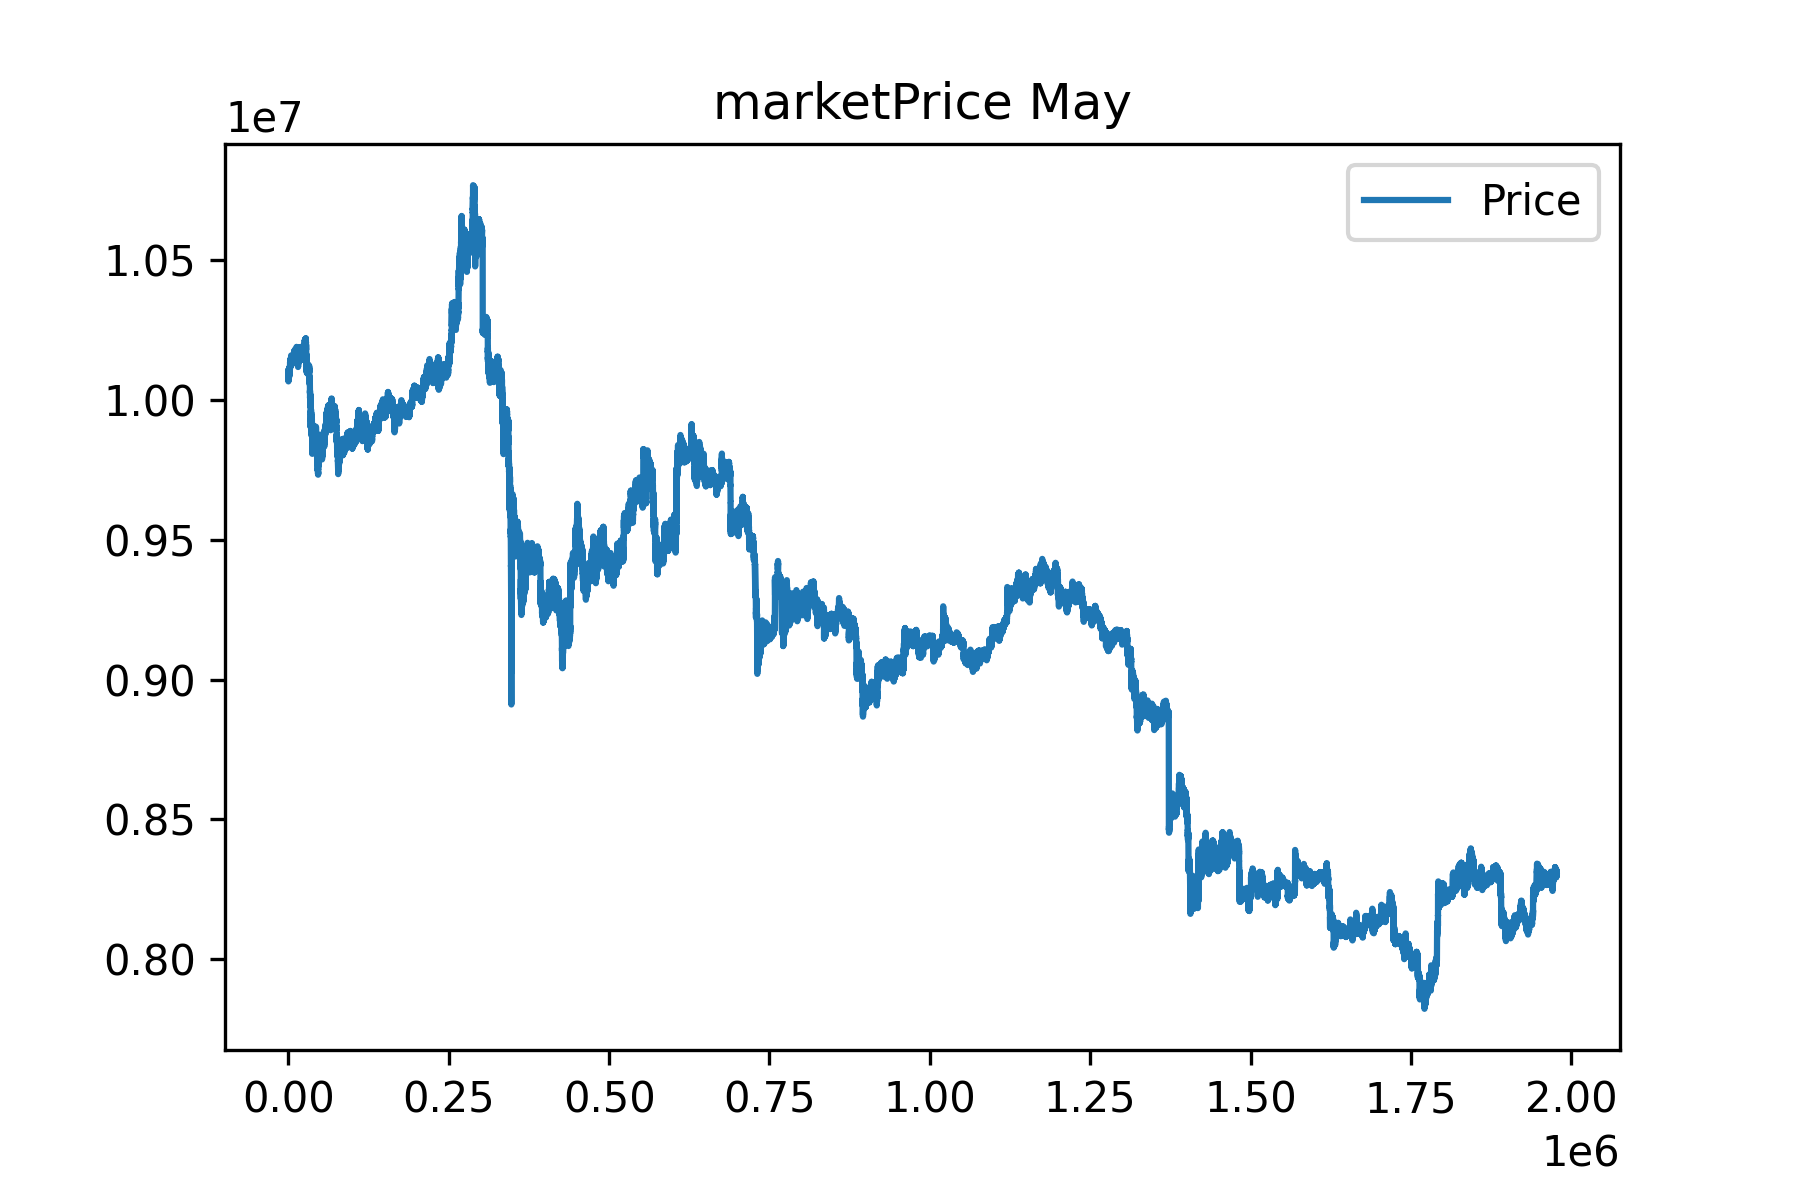
\includegraphics[scale=0.4]{marketPriceMay.png}}
\caption{Time-market price graph.}
\label{fig}
\end{figure}

Our market price analysis (Fig.\ref{fig}) shows each second's market price by timeline. 

\subsection{Daily market price and transaction count}

\begin{figure}[htbp]
\centering
\subfigure[\label{fig:daily_market_price}]{
  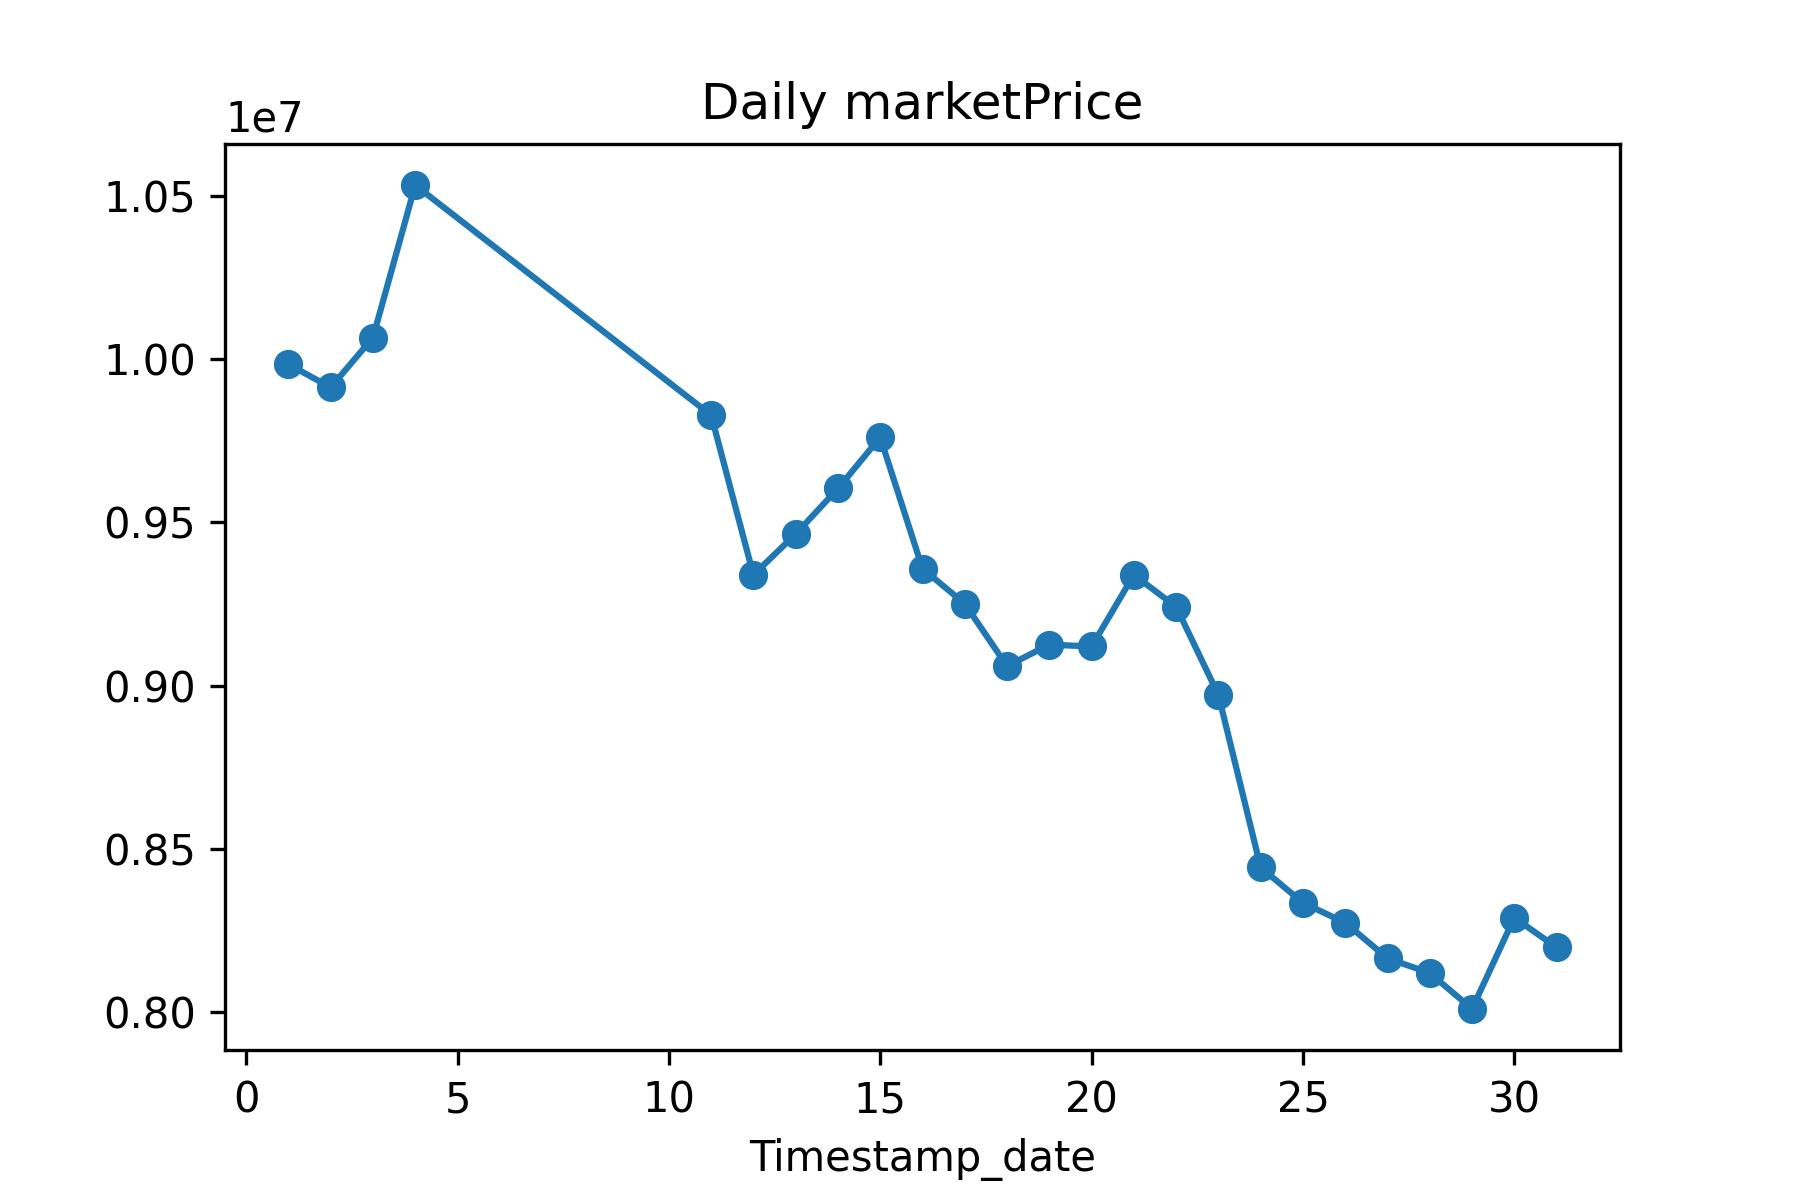
\includegraphics[width=2.5in]{dailyMarketPrice.png}
}
\subfigure[\label{fig:transaction_count_per_day}]{
  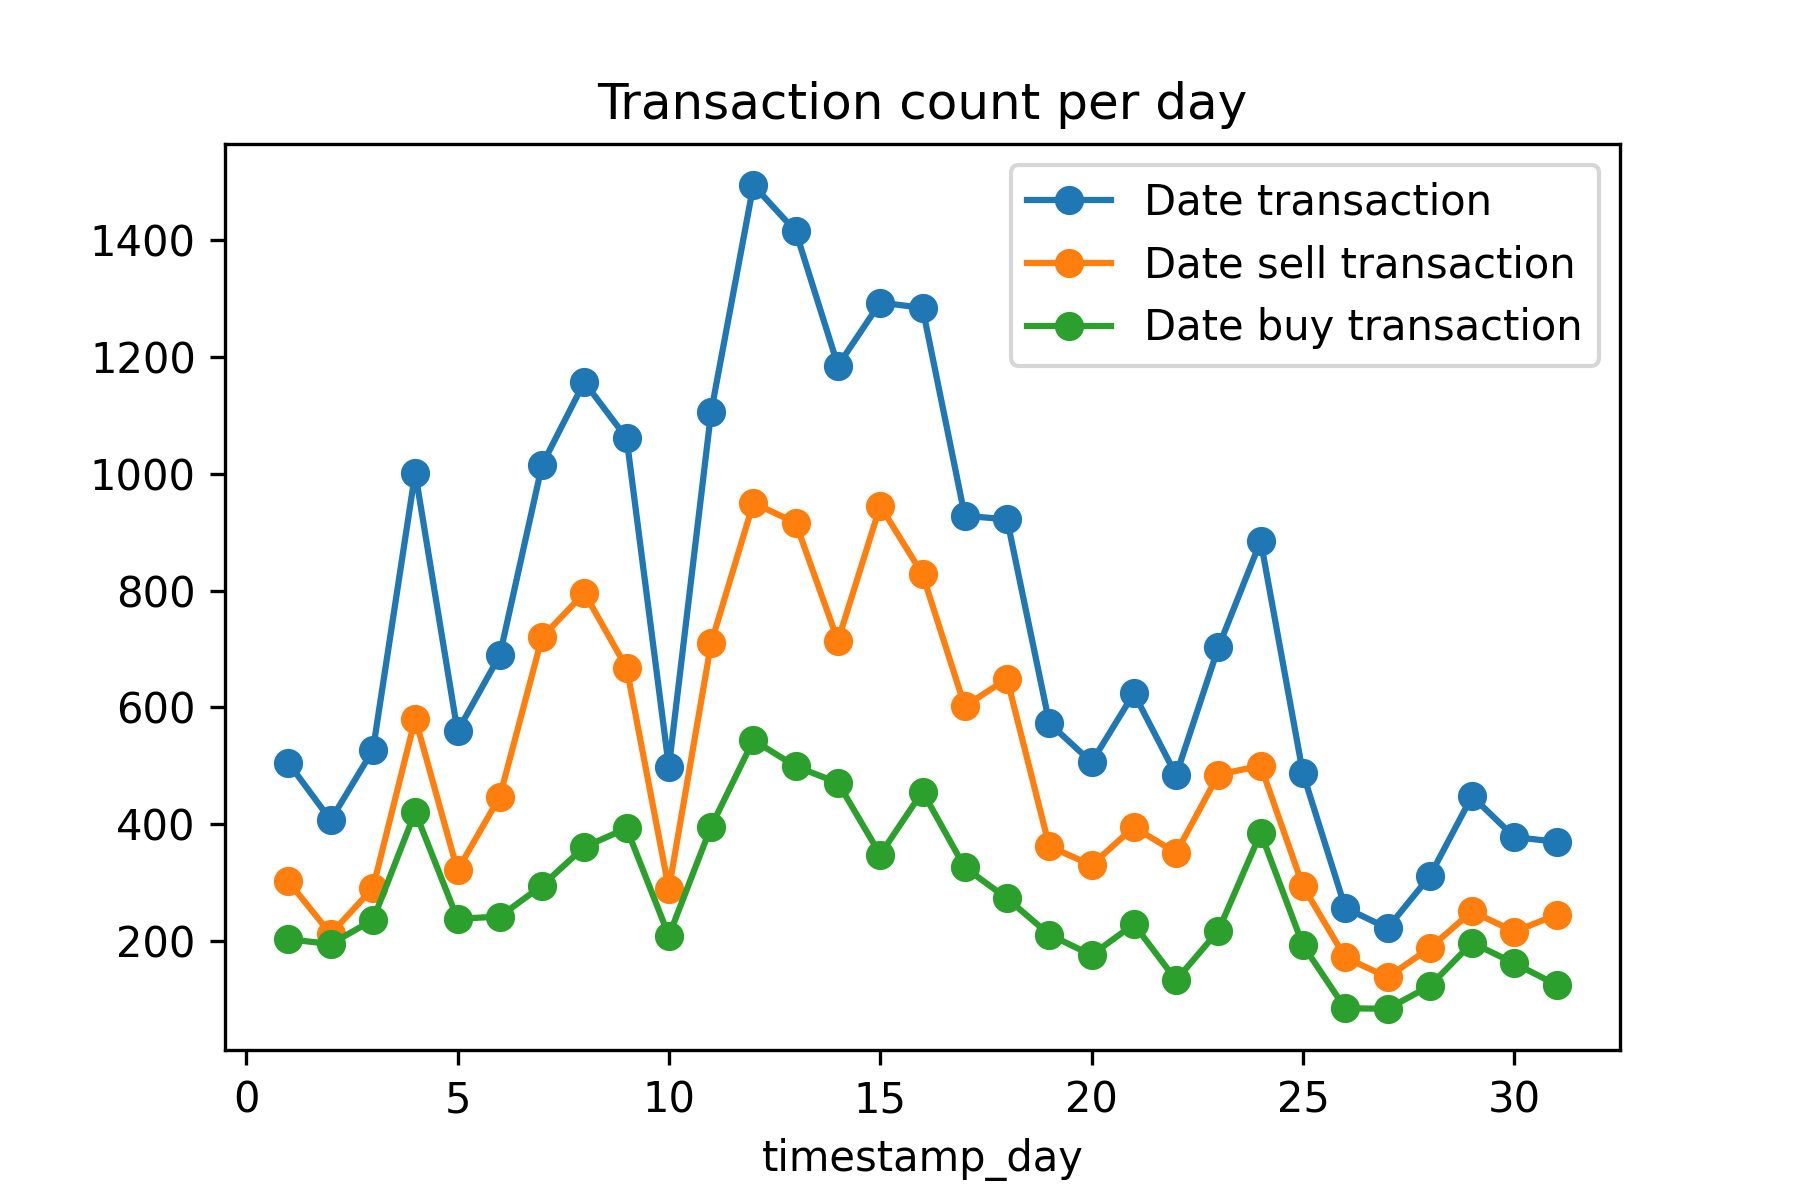
\includegraphics[width=2.5in]{Transaction_count_per_day.png}
}
\caption{(a) date-market price graph; (b) date-transaction graph}
\label{fig:daily}
\vspace{-0.5cm}
\end{figure}

\begin{itemize}
\item Our daily market price analysis (Fig.\ref{fig:daily}-(a)) shows each day's mean of market price. Daily market price graph shows similar shape with market price graph (Fig.\ref{fig})
\item Our transaction count per day analysis (Fig.\ref{fig:daily}-(b)) shows each day's selling transaction, buying transaction, and total transaction. Every each day, selling transaction amount is larger than buying transaction amount. Maybe it means each selling transaction's scale is smaller than that of buying transactions.
\end{itemize}

\subsection{Hourly market price and transaction count}

\begin{figure}[htbp]
\centering
\subfigure[\label{fig:hourly_market_price}]{
  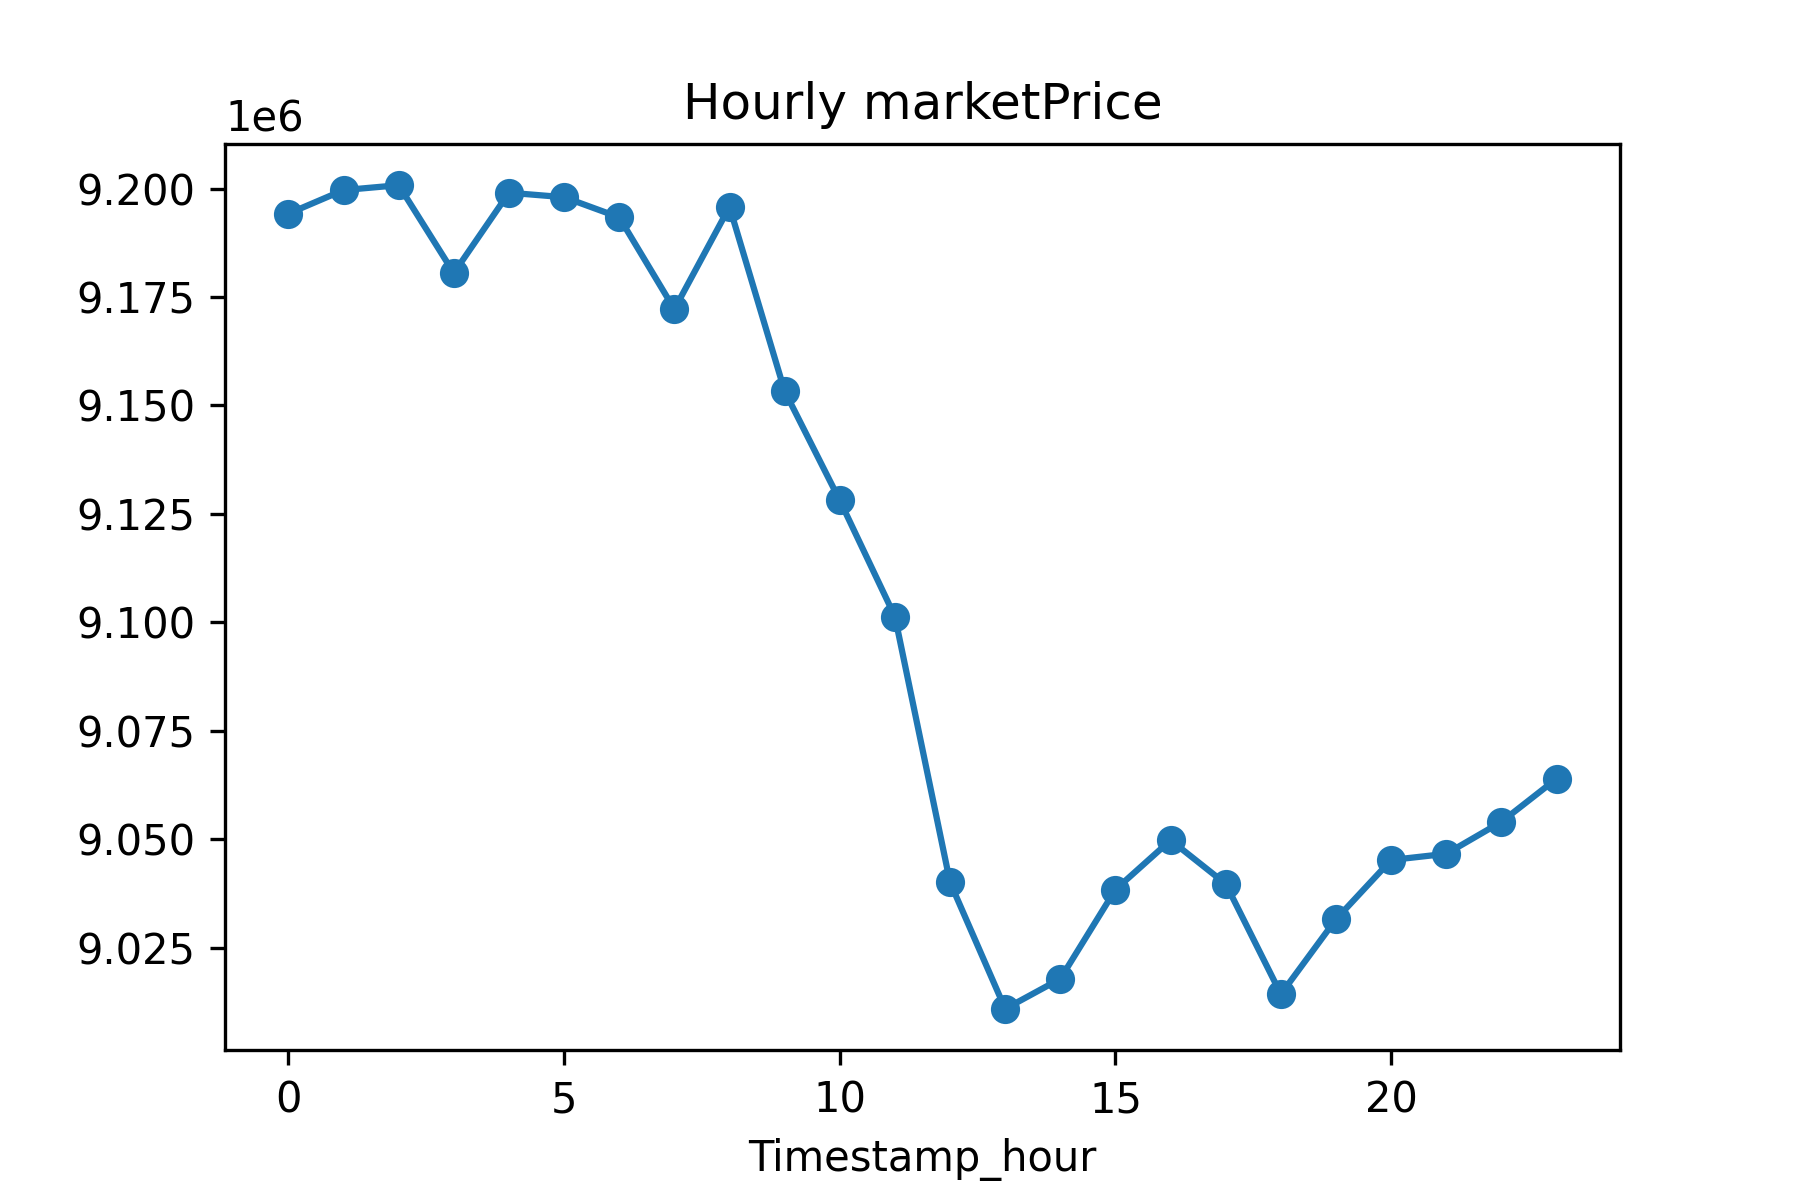
\includegraphics[width=2.5in]{hourlyMarketPrice.png}
}
\subfigure[\label{fig:hourly_transaction_count}]{
  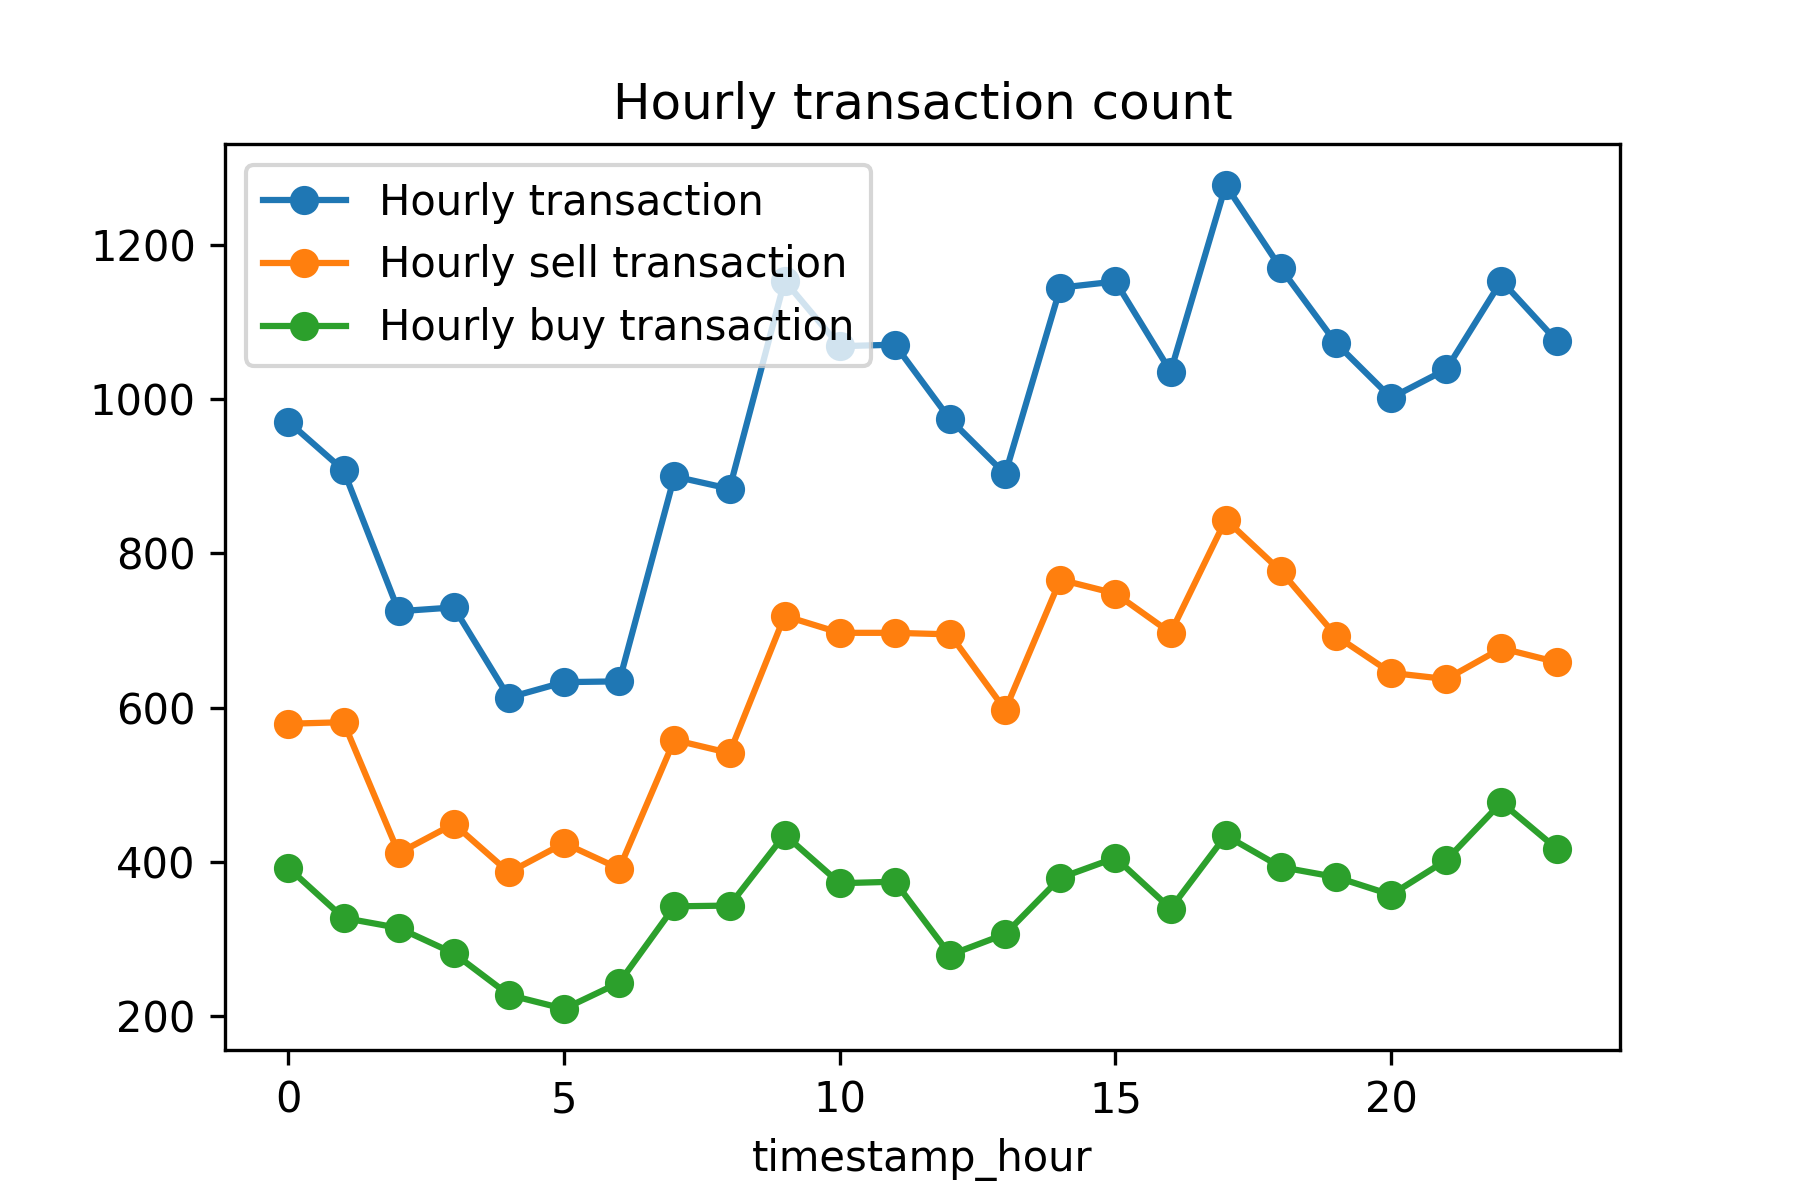
\includegraphics[width=2.5in]{Hourly transaction count.png}
}
\caption{(a) hour-market price graph; (b) hour-transaction graph}
\label{fig:hour}
\vspace{-0.5cm}
\end{figure}

\begin{itemize}
\item Our hourly market price analysis (Fig.\ref{fig:hour}-(a)) shows each hour's mean of market price. The market price is relatively high in the morning, and the market price tends to drop in the afternoon. 
\item Our transaction count per day analysis (Fig.\ref{fig:hour}-(b)) shows each hour's selling transaction, buying transaction, and total transaction. Every each hour, selling transaction amount is larger than buying transaction amount. Maybe it means each selling transaction's scale is smaller than that of buying transactions.
\item The market price is relatively high in the morning, and the market price tends to drop in the afternoon. Conversely, transaction counts tend to be low in the morning and high in the afternoon. Therefore, transaction count and market price are inversely proportional.
\end{itemize}

\subsection{Minute market price and transaction count}

\begin{figure}[htbp]
\centering
\subfigure[\label{fig:minute_market_price}]{
  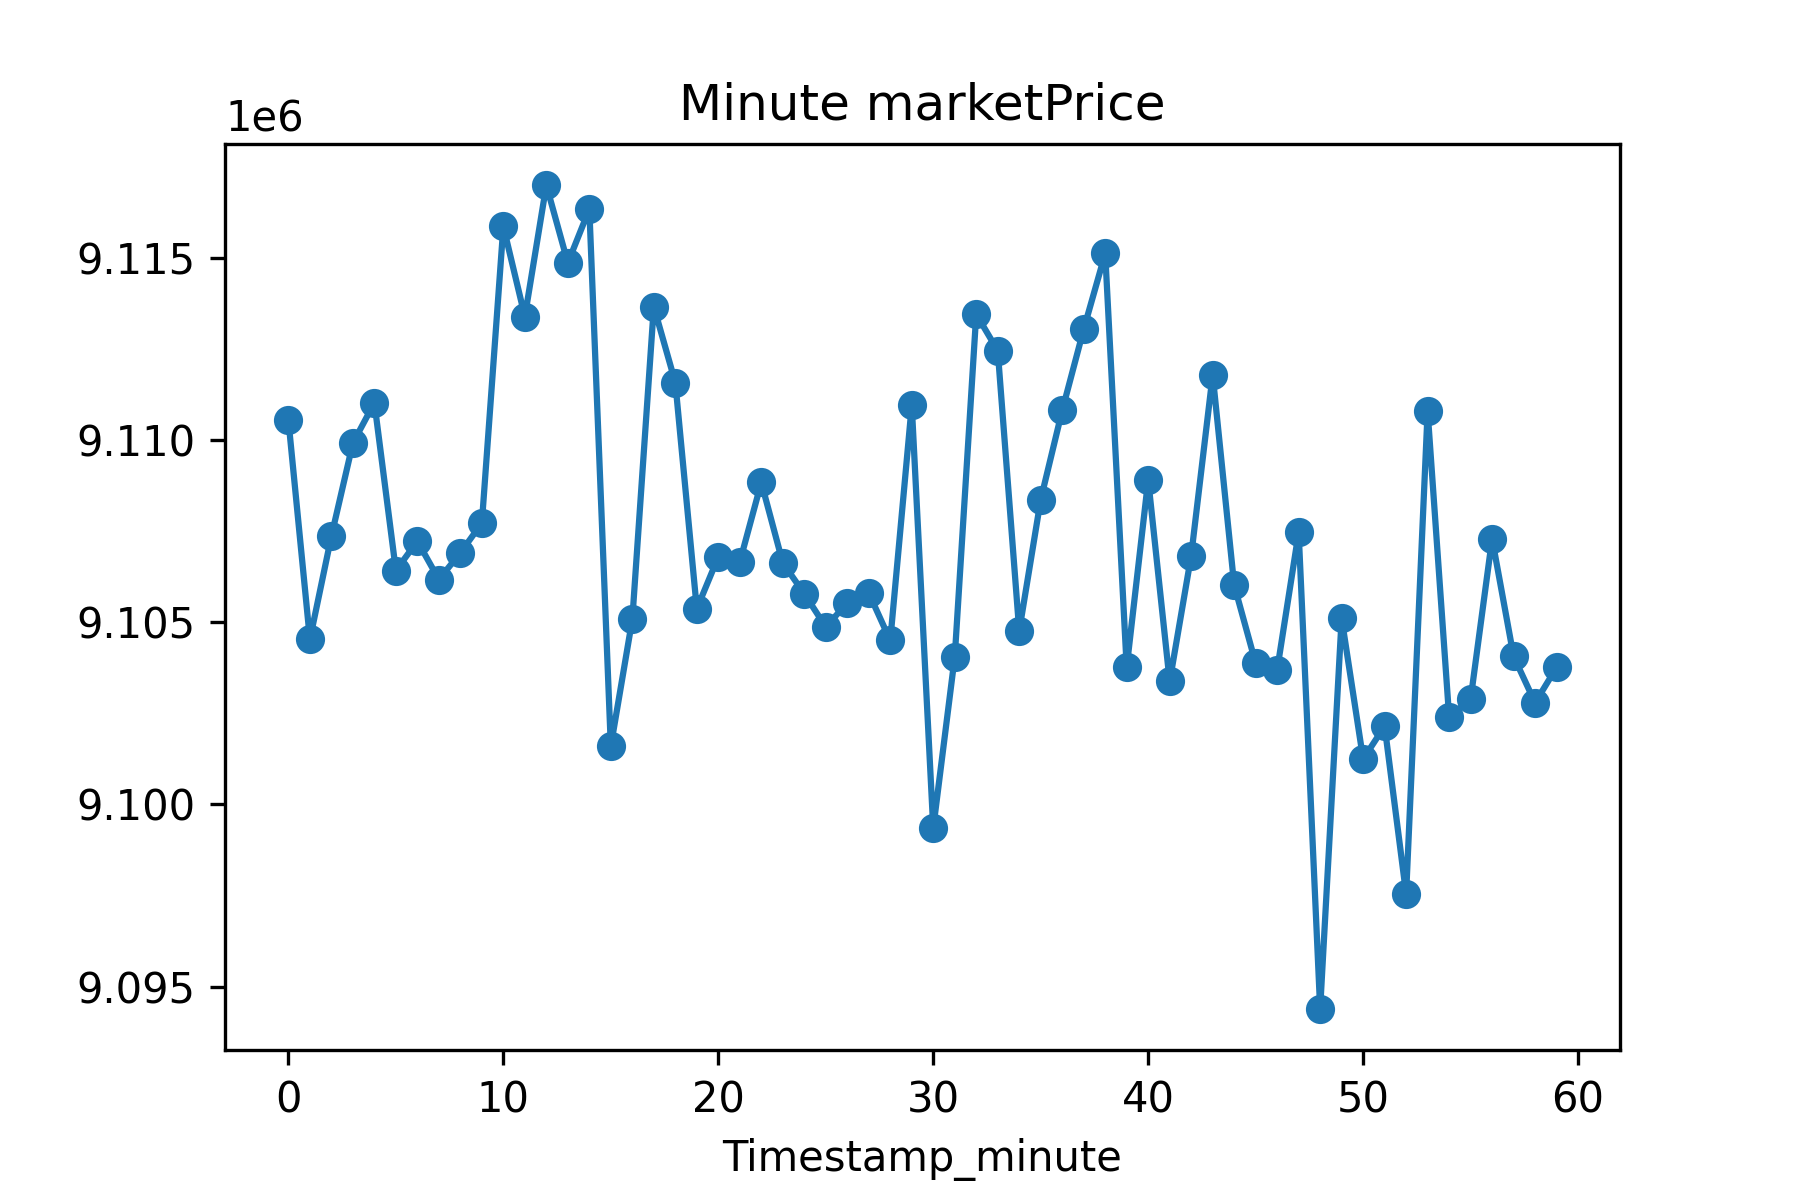
\includegraphics[width=2.5in]{minuteMarketPrice.png}
}
\subfigure[\label{fig:transaction_count_per_minute}]{
  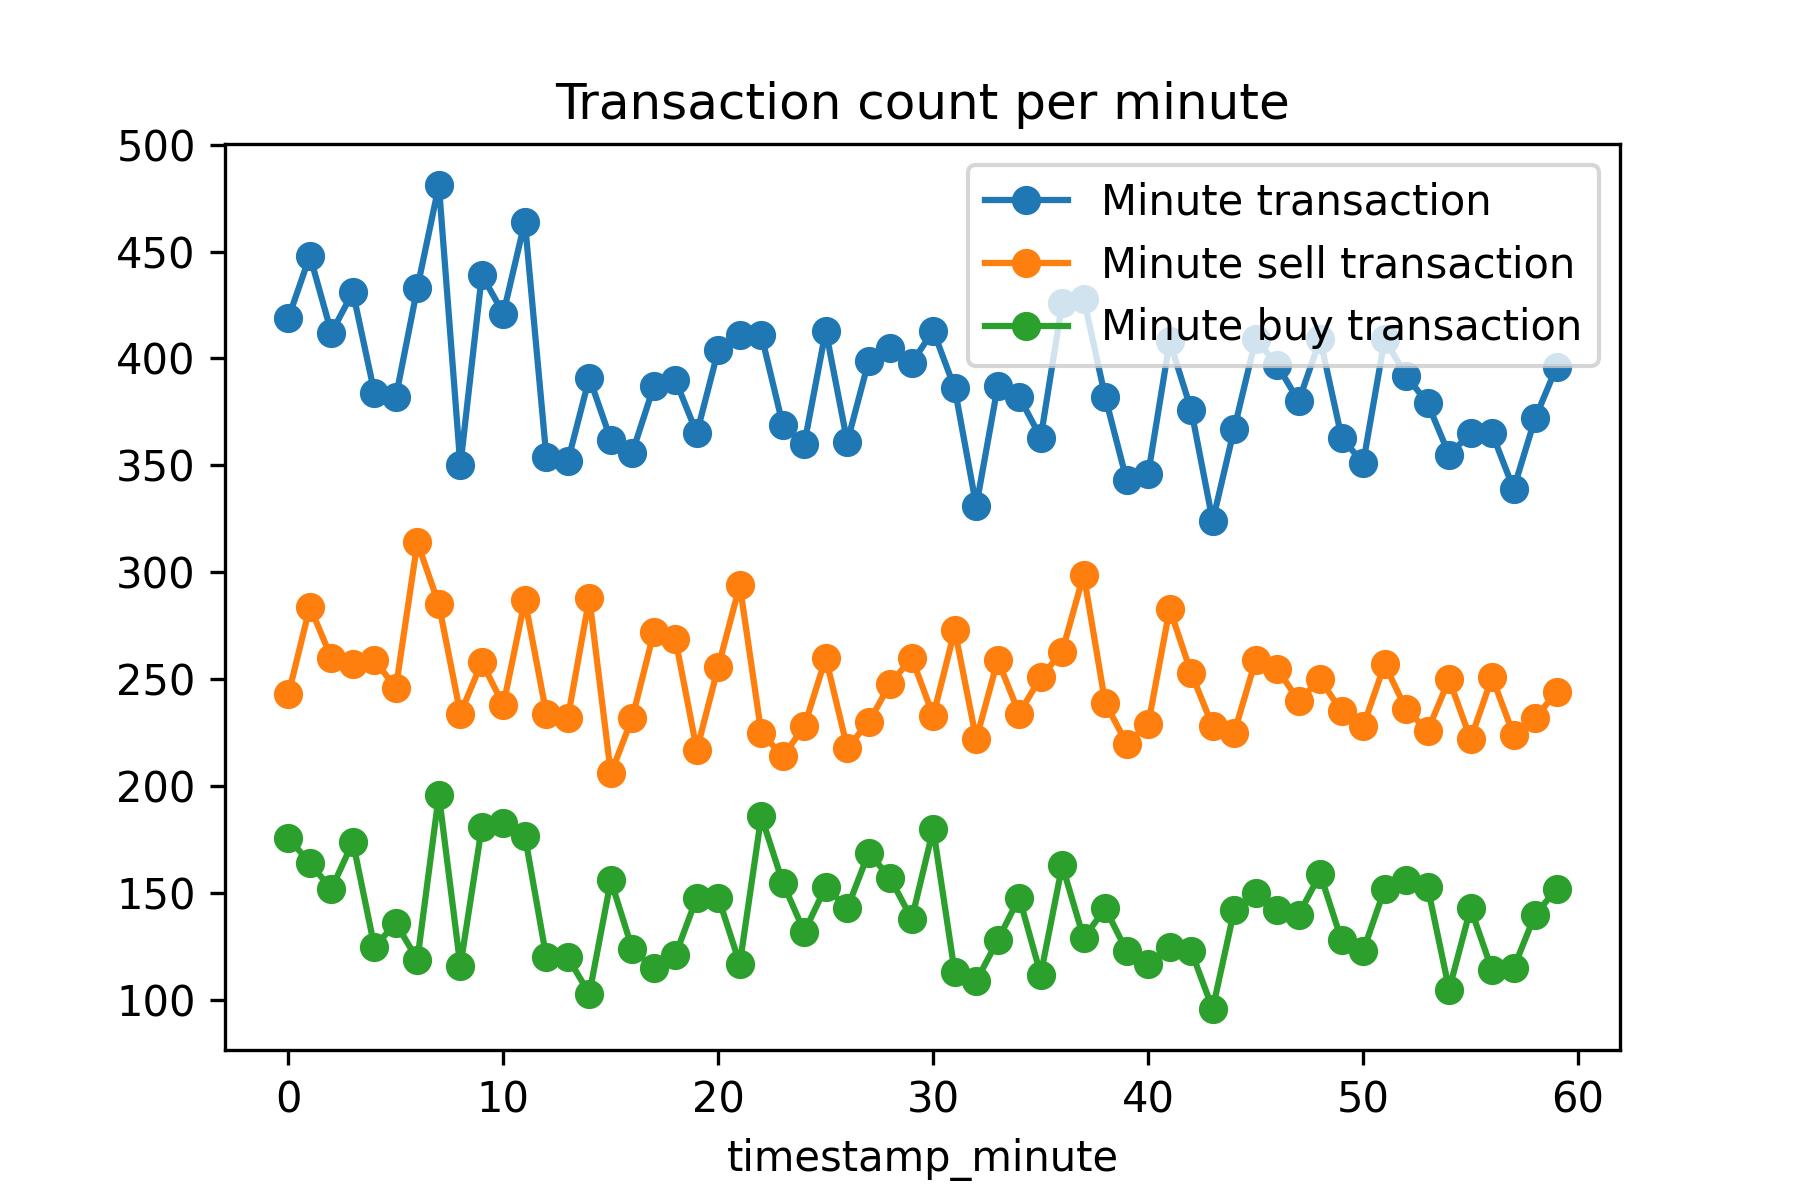
\includegraphics[width=2.5in]{Transaction_count_per_minute.png}
}
\caption{(a) minute-market price graph; (b) minute-transaction graph}
\label{fig:minute}
\vspace{-0.5cm}
\end{figure}

\begin{itemize}
\item Our market price by minute analysis (Fig.\ref{fig:minute}-(a)) shows each minute's mean of market price. 
\item Our transaction count per minute analysis (Fig.\ref{fig:minute}-(b)) shows each minute's selling transaction, buying transaction, and total transaction. Every each minute, selling transaction amount is larger than buying transaction amount. Maybe it means each selling transaction's scale is smaller than that of buying transactions.
\end{itemize}

\subsection{Profit analyze}

\begin{figure}[htbp]
\centering
\subfigure[\label{fig:profit_graph}]{
  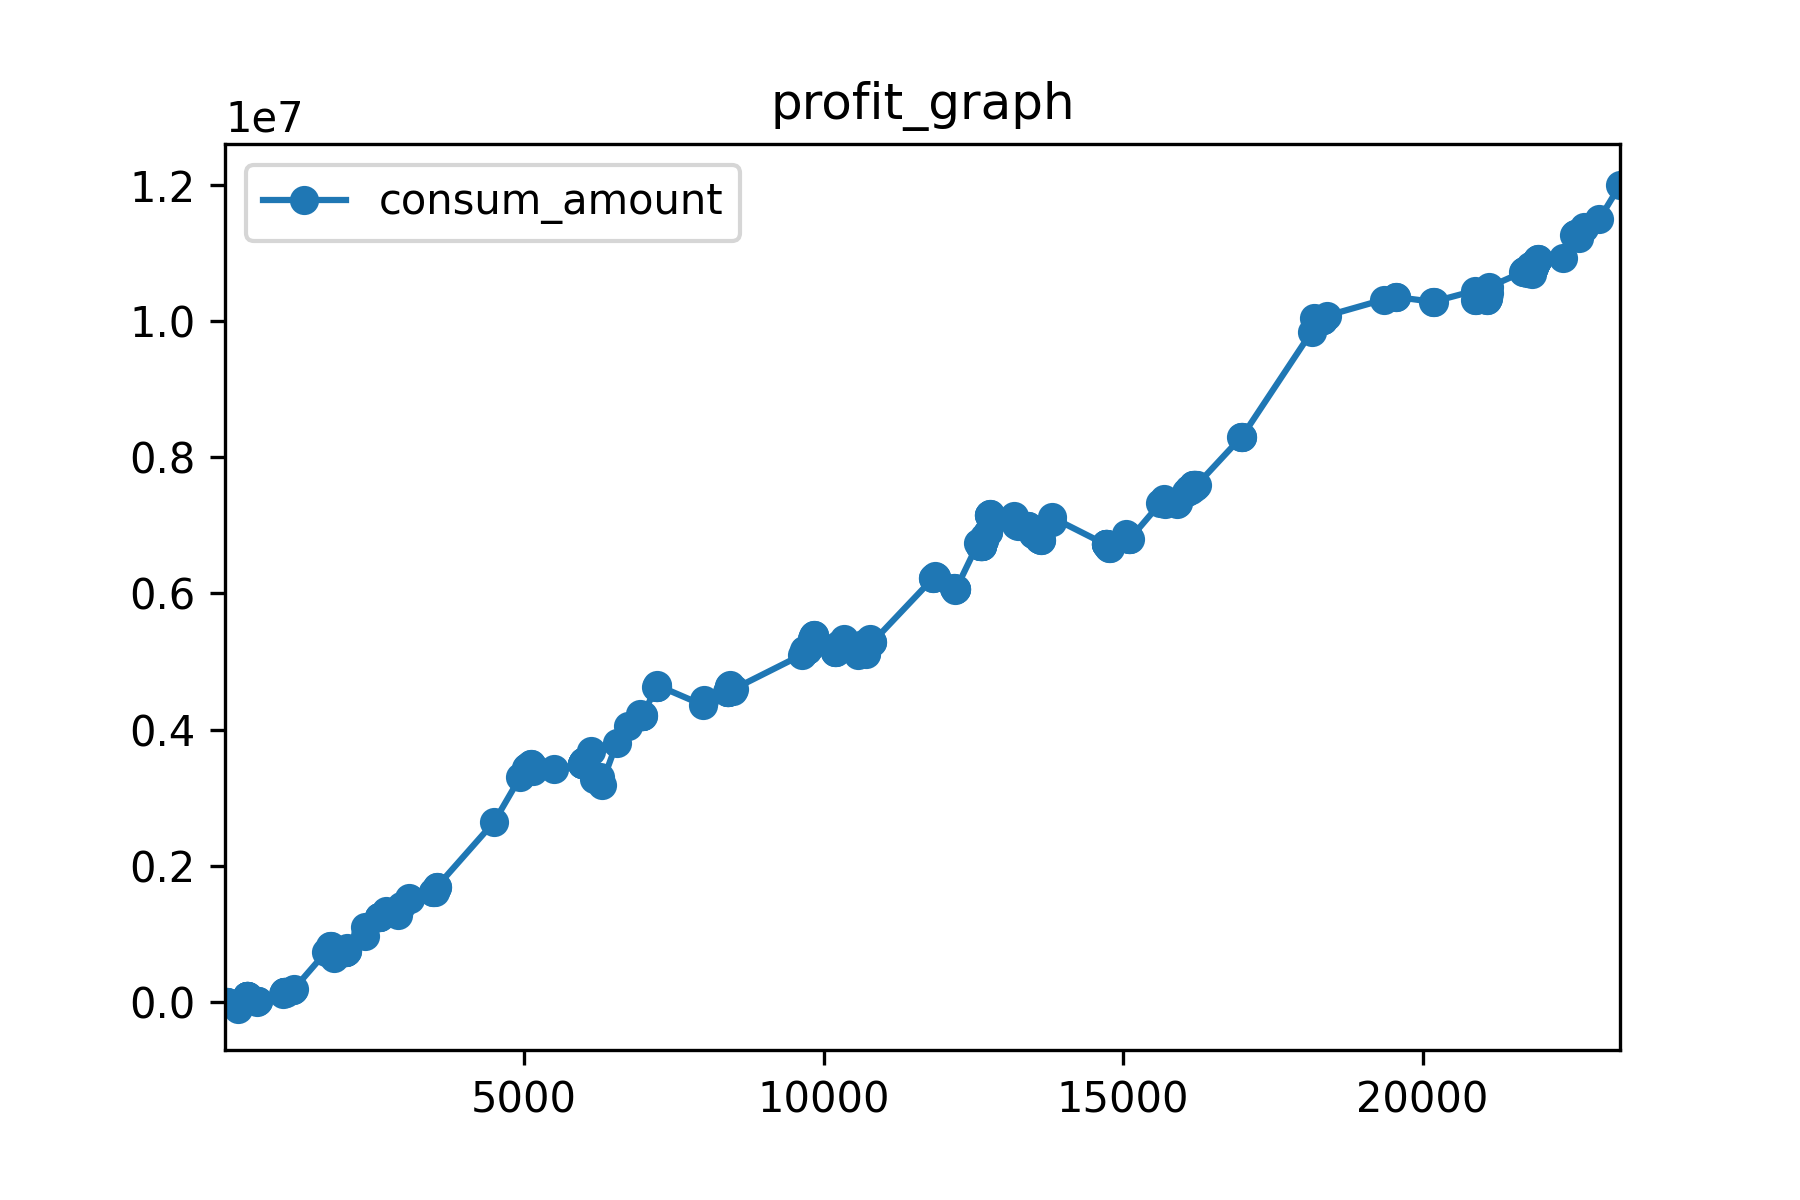
\includegraphics[width=2.5in]{profit_graph.png}
}
\subfigure[\label{fig:profit_point_graph}]{
  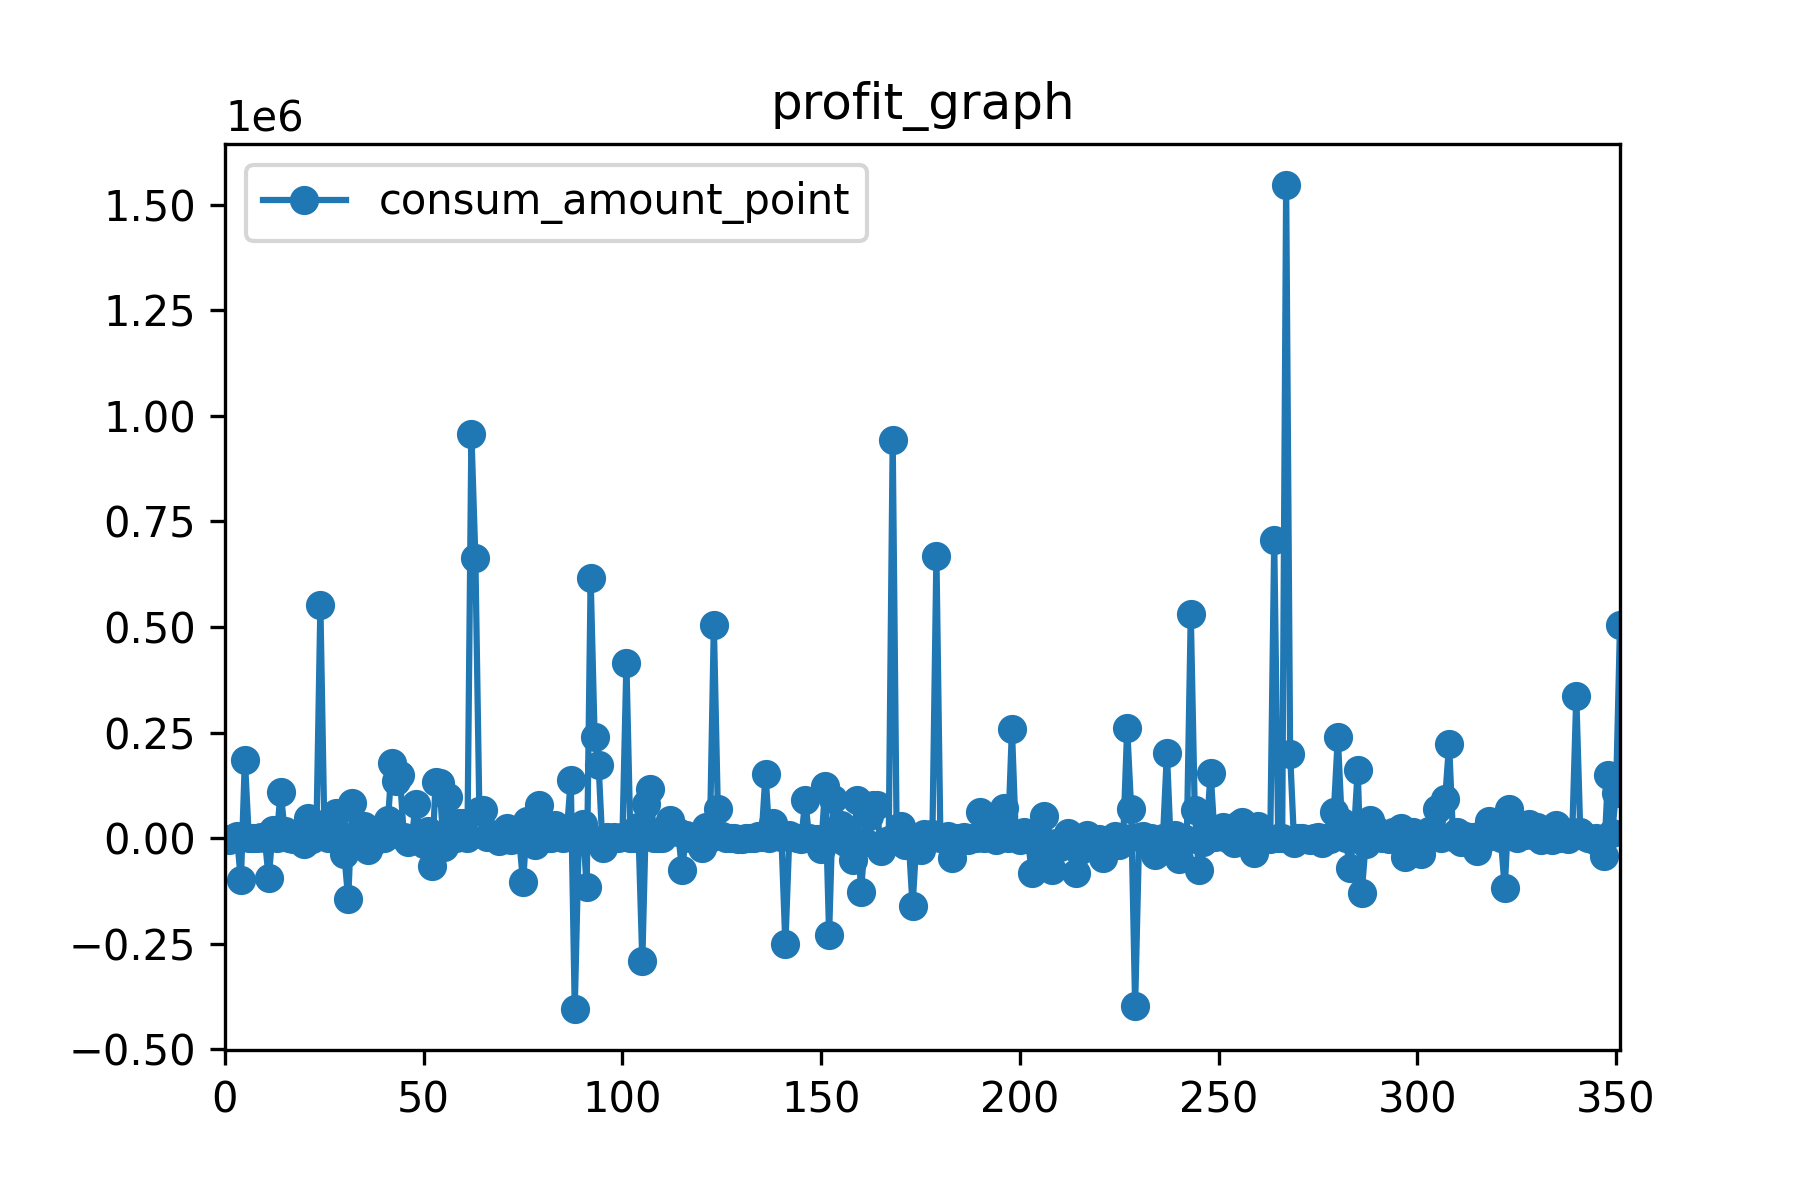
\includegraphics[width=2.5in]{profit_point_graph.png}
}
\caption{(a) time-profit graph (accumulative); (b) time-profit graph (by section)}
\label{fig:profit}
\vspace{-0.5cm}
\end{figure}

\begin{itemize}
\item Our market price by minute analysis (Fig.\ref{fig:profit}-(a)) shows 
\item Our transaction count per minute analysis (Fig.\ref{fig:profit}-(b)) shows each 
\end{itemize}

\section*{Tables}

\begin{itemize}

\item Transaction average, minimum, maximum table \href{https://github.com/kimsangwond/bithumb_bot/blob/master/sangw on_code/table/avg%2C%20min%2C%20max_table.csv}{(link)}

\item 
Profit table (accumulated) \href{https://github.com/kimsangwond/bithumb_bot/blob/master/sangw on_code/table/profit_table.csv}{(link)}

\item 
Profit table (by section) \href{https://github.com/kimsangwond/bithumb_bot/blob/master/sangw on_code/table/profit_table2.csv}{(link)}

\item 
Profit table (by section) \href{https://github.com/kimsangwond/bithumb_bot/blob/master/sangw on_code/table/profit_table2.csv}{(link)}

\item 
Date-market price table \href{https://github.com/kimsangwond/bithumb_bot/blob/master/hamin _code/table/date_result_table.csv}{(link)}

\item 
Hour-market price table \href{https://github.com/kimsangwond/bithumb_bot/blob/master/hamin _code/table/hour_result_table.csv}{(link)}

\item 
Minute-market price table \href{https://github.com/kimsangwond/bithumb_bot/blob/master/hamin
_code/table/minute_result_table.csv}{(link)}
\end{itemize}

\section*{Acknowledgment}

The preferred spelling of the word ``acknowledgment'' in America is without 
an ``e'' after the ``g''. Avoid the stilted expression ``one of us (R. B. 
G.) thanks $\ldots$''. Instead, try ``R. B. G. thanks$\ldots$''. Put sponsor 
acknowledgments in the unnumbered footnote on the first page.

\section*{References}

Please number citations consecutively within brackets \cite{b1}. The 
sentence punctuation follows the bracket \cite{b2}. Refer simply to the reference 
number, as in \cite{b3}---do not use ``Ref. \cite{b3}'' or ``reference \cite{b3}'' except at 
the beginning of a sentence: ``Reference \cite{b3} was the first $\ldots$''

Number footnotes separately in superscripts. Place the actual footnote at 
the bottom of the column in which it was cited. Do not put footnotes in the 
abstract or reference list. Use letters for table footnotes.

Unless there are six authors or more give all authors' names; do not use 
``et al.''. Papers that have not been published, even if they have been 
submitted for publication, should be cited as ``unpublished'' \cite{b4}. Papers 
that have been accepted for publication should be cited as ``in press'' \cite{b5}. 
Capitalize only the first word in a paper title, except for proper nouns and 
element symbols.

For papers published in translation journals, please give the English 
citation first, followed by the original foreign-language citation \cite{b6}.

\begin{thebibliography}{00}
\bibitem{b1} G. Eason, B. Noble, and I. N. Sneddon, ``On certain integrals of Lipschitz-Hankel type involving products of Bessel functions,'' Phil. Trans. Roy. Soc. London, vol. A247, pp. 529--551, April 1955.
\bibitem{b2} J. Clerk Maxwell, A Treatise on Electricity and Magnetism, 3rd ed., vol. 2. Oxford: Clarendon, 1892, pp.68--73.
\bibitem{b3} I. S. Jacobs and C. P. Bean, ``Fine particles, thin films and exchange anisotropy,'' in Magnetism, vol. III, G. T. Rado and H. Suhl, Eds. New York: Academic, 1963, pp. 271--350.
\bibitem{b4} K. Elissa, ``Title of paper if known,'' unpublished.
\bibitem{b5} R. Nicole, ``Title of paper with only first word capitalized,'' J. Name Stand. Abbrev., in press.
\bibitem{b6} Y. Yorozu, M. Hirano, K. Oka, and Y. Tagawa, ``Electron spectroscopy studies on magneto-optical media and plastic substrate interface,'' IEEE Transl. J. Magn. Japan, vol. 2, pp. 740--741, August 1987 [Digests 9th Annual Conf. Magnetics Japan, p. 301, 1982].
\bibitem{b7} M. Young, The Technical Writer's Handbook. Mill Valley, CA: University Science, 1989.
\end{thebibliography}
\vspace{12pt}
\color{red}
IEEE conference templates contain guidance text for composing and formatting conference papers. Please ensure that all template text is removed from your conference paper prior to submission to the conference. Failure to remove the template text from your paper may result in your paper not being published.

\end{document}
